%% =====================================================================
%%  Explainable Adaptive Continuous Authentication for Smart Healthcare
%%  IEEEtran conference format.  Compile on Overleaf with pdfLaTeX:
%%      pdflatex -> bibtex -> pdflatex -> pdflatex
%% =====================================================================
\documentclass[conference]{IEEEtran}
\IEEEoverridecommandlockouts

\usepackage{cite}
\usepackage{amsmath,amssymb,amsfonts}
\usepackage{algorithm}
\usepackage{algpseudocode}
\usepackage{graphicx}
\usepackage{textcomp}
\usepackage{xcolor}
\usepackage{booktabs}
\usepackage{array}
\usepackage{multirow}
\usepackage{threeparttable}
\usepackage{url}
\usepackage{tikz}
\usepackage{relsize}
\usepackage{balance}
\usetikzlibrary{arrows.meta,positioning,fit,calc,shapes.geometric,backgrounds}
\usepackage[hidelinks,breaklinks]{hyperref}

\newcommand{\allow}{\textsc{allow}}
\newcommand{\otp}{\textsc{otp}}
\newcommand{\strongauth}{\textsc{strong}}
\newcommand{\deny}{\textsc{deny}}
\setlength{\tabcolsep}{3.2pt}
\newcommand{\tablepath}[1]{tables/#1}
\newcommand{\figpath}[1]{figures/#1}

\begin{document}

\title{Explainable Adaptive Continuous Authentication for\\
Smart Healthcare: Exact Inline Attribution and a\\
Clinical Safety Valve under Zero Trust}

\author{\IEEEauthorblockN{Ritesh Mukherjee}
\IEEEauthorblockA{\textit{Department of Computing and Mathematics} \\
\textit{Manchester Metropolitan University}\\
Manchester, United Kingdom \\
25929520@stu.mmu.ac.uk}
}

\maketitle

\begin{abstract}
Healthcare has led every industry in average breach cost for more than a
decade, and the two largest recent incidents in the sector both began with
credentials that were valid at the point of entry and were never re-verified
afterwards. Continuous authentication addresses precisely this failure, but
the two literatures that could supply it are each incomplete: reinforcement
learning risk engines adapt well yet cannot justify their decisions, while
explainable-AI authentication produces readable attributions on fixed corpora
and explains only after the fact. Neither prices the distinctive cost of the
clinical setting, where obstructing a legitimate clinician is a patient-safety
event rather than a usability nuisance. We develop the Hybrid Explainable
Adaptive Authentication Framework (HEAAF) and evaluate it on a testbed whose
behavioural channel is the real CMU keystroke-dynamics benchmark, extended
with generated clinical context and six labelled attack scenarios traceable to
documented incidents. We report three results and one refutation. First, the
explanation a clinician receives need not be an approximation at all: because
sixteen evidence features partition into eight semantic groups, exact
group-level Shapley values cost $2^{8}=256$ coalition evaluations and run in
$0.44$\,ms, so a complete end-to-end decision with an \emph{exact} justification
takes $0.61$\,ms --- faster than the same decision with approximate integrated
gradients. We also show that the common practice of summing feature
attributions into groups is not the group Shapley value, and measure the
resulting disagreement ($\rho=0.93$). Second, an explicit clinical safety valve
removes emergency denials entirely: holding the detector and the friction
budget fixed, denials under declared emergency fall from $1.10\%$ to
$0.000\%$ for a G-mean cost of $0.005$ $[0.002, 0.009]$, and the graded
escalation ladder delivers the same detection for $7.6$ rather than $26.5$
clinician-hours of annual friction. Third, and contrary to our starting
hypothesis, the reinforcement-learning risk score is \emph{not} the strongest
detector: a supervised detector inside the same policy engine gains $0.378$
$[0.283,0.469]$ G-mean. We conclude that the contribution of RL here lies in
the graded action policy rather than in scoring, and report the negative result
in full.
\end{abstract}

\begin{IEEEkeywords}
continuous authentication, explainable AI, Shapley values, zero trust
architecture, smart healthcare, Internet of Medical Things, reinforcement
learning, keystroke dynamics
\end{IEEEkeywords}

\section{Introduction}

Smart healthcare couples electronic health records (EHRs), Internet of Medical
Things (IoMT) devices, telemedicine and cloud platforms into a single
data-driven care pathway, and in the United Kingdom the NHS sits at the centre
of national critical infrastructure on that basis~\cite{nhsdspt}. The same
integration widens the attack surface. IBM's 2025 analysis places healthcare at
the top of the breach-cost table for the fourteenth consecutive year, at an
average of USD~7.42~million per breach, with a mean of 279 days to identify and
contain~\cite{ibm2025}. Credentials remain the dominant entry
vector~\cite{verizon2025}.

Two incidents define the problem this paper addresses. In February 2024,
attackers entered Change Healthcare through a remote-access portal that did not
enforce multi-factor authentication, using valid credentials, and then moved
laterally for nine days before deploying ransomware; the resulting breach
affected an estimated 192.7~million individuals. In June 2024, the Qilin group
encrypted systems at Synnovis, the pathology provider for two large London NHS
trusts; NHS England recorded delays to over 11,000 outpatient and elective
appointments~\cite{nhssynnovis}, 1,710 operations were postponed, and King's
College Hospital NHS Foundation Trust subsequently confirmed that the
disruption contributed to a patient death.

The common structure is that authentication was a gate rather than a process.
Once the gate was passed, nothing re-verified the identity behind the session
while it enumerated records for days. This is exactly the failure the NIST Zero
Trust Architecture (ZTA) model is designed to eliminate by requiring that
access decisions be re-evaluated continuously from identity, behaviour and
environmental signal~\cite{nist800207,syed2022}.

Two research directions supply components of such a system, and neither is
deployable in a hospital on its own.

\begin{itemize}
\item \textbf{Reinforcement-learning risk engines.} RLAuth adapts the
authentication challenge to contextual risk and reports a G-mean of
$92.62\%$~\cite{rlauth}; Bansal and Ouda show that keystroke dynamics support
continuous verification via a deep Q-network~\cite{bansal2024}. Both are
opaque. Notably, the authors of RLAuth observe that their system cannot detect
attacks mounted from \emph{known} environments, such as a colleague at a
familiar workstation~\cite{rlauth} --- which is exactly the insider case that
dominates healthcare enforcement action.
\item \textbf{Explainable authentication.} Abdel Raouf et al.\ combine CTGAN
augmentation with LIME for keystroke authentication~\cite{raouf2024}, and Mohd
Nizam et al.\ apply SHAP and LIME to touch-stroke continuous
authentication~\cite{nizam2026}. In both, explanation is post-hoc and evaluated
on a closed corpus, with no adaptive control loop.
\end{itemize}

A third gap belongs to neither literature. In a clinical environment the cost
of a false challenge is not symmetric with the cost of a missed detection, and
it is not constant: interrupting a billing query and interrupting a
resuscitation are different events. Koppel et al.'s ethnography of clinician
workarounds documents the consequence when this is ignored --- staff share
credentials, defeat logout and route around controls, because the controls were
designed without reference to clinical tempo~\cite{koppel2015}. Any
authentication policy that treats friction as a scalar nuisance will reproduce
that outcome.

\subsection{Contributions}

\begin{enumerate}
\item We specify HEAAF as a four-layer architecture mapped onto the NIST ZTA
policy engine / policy administrator / policy enforcement point decomposition,
with a \emph{clinical safety valve} that makes patient-safety cost an explicit
term in the decision rather than an afterthought (Section~\ref{sec:framework}).

\item We show that the explanation disclosed to a clinician can be \emph{exact}
rather than approximate. The sixteen evidence features partition into eight
semantic groups, so the group game admits exact Shapley values at $2^{8}=256$
coalition evaluations; measured at $0.44$\,ms, a full decision with an exact
justification costs $0.61$\,ms end to end, which is \emph{cheaper} than the
same decision explained by approximate integrated gradients
(Section~\ref{sec:results-edl}). We further show, and verify numerically, that
summing feature-level Shapley values within a block is not the Shapley value of
that block in the quotient game whenever interactions of order three or above
straddle groups unevenly (Section~\ref{sec:edl}).

\item We isolate the clinical safety valve with detector and friction budget
held fixed, and quantify what the graded escalation ladder buys: identical
detection at $3.5\times$ lower annual clinician-hour cost, because escalation
substitutes an eight-second challenge for a forty-five-second denial
(Section~\ref{sec:results-policy}).

\item We report a negative result in full: the RL-derived risk score is
outperformed on detection by a supervised detector operating inside the same
policy engine, with a paired bootstrap interval that excludes zero by a wide
margin. This relocates the contribution of RL to the action layer
(Section~\ref{sec:results-policy}).

\item We analyse the explanation channel as an attack surface and implement
role-scoped disclosure, quantifying what each audience receives
(Section~\ref{sec:security}).

\item We release the full pipeline, an invariant test suite that mechanically
checks the axioms and safety properties the argument depends on, and scripts
that regenerate every table and figure from the persisted results
(Section~\ref{sec:repro}).
\end{enumerate}

\subsection{A note on a corrected earlier configuration}
\label{sec:correction}

An earlier revision of this work injected a supervised gradient-boosting score
as a seventeenth input feature shared by every policy. That configuration is
withdrawn. It placed a supervised detector underneath both the
reinforcement-learning agent and the supervised baseline it is compared with,
which makes the central comparison of this paper uninterpretable; measured on
held-out data it also \emph{degraded} the supervised detector
(AUROC $0.931$ with the extra feature, $0.949$ without). Every policy reported
here consumes the same sixteen interpretable evidence features. Removing the
stacked feature weakens the RL score --- which is the direction that makes our
negative result harder for us, not easier --- and we report it on that basis.

\section{Related Work and Positioning}
\label{sec:related}

\begin{table*}[t]
\centering
\caption{Positioning against representative prior work. ``Inline'' means the
explanation is produced within the decision cycle rather than reconstructed
afterwards; ``exact'' means the disclosed attribution is a Shapley value
computed over all coalitions rather than sampled or approximated.}
\label{tab:related}
\small
\begin{tabular}{lccccccc}
\toprule
System & Adaptive & Graded & Explains & Inline & Exact & Clinical & Evaluation \\
 & policy & actions & decisions & expl. & expl. & cost model & data \\
\midrule
RLAuth~\cite{rlauth} & \checkmark & \checkmark & --- & --- & --- & --- & synthetic contexts \\
Bansal \& Ouda~\cite{bansal2024} & \checkmark & --- & --- & --- & --- & --- & keystroke corpus \\
Freeman et al.~\cite{freeman2016} & \checkmark & \checkmark & partial & \checkmark & --- & --- & production logins \\
Wiefling et al.~\cite{wiefling2022} & \checkmark & \checkmark & --- & --- & --- & --- & 31.3M logins \\
Abdel Raouf et al.~\cite{raouf2024} & --- & --- & \checkmark & --- & --- & --- & keystroke corpus \\
Mohd Nizam et al.~\cite{nizam2026} & --- & --- & \checkmark & --- & --- & --- & touch corpus \\
FastSHAP~\cite{jethani2022} & n/a & n/a & \checkmark & \checkmark & --- & n/a & vision/tabular \\
\midrule
\textbf{HEAAF} (this work) & \checkmark & \checkmark & \checkmark & \checkmark & \checkmark & \checkmark & real keystroke + \\
 & & & & & & & generated context \\
\bottomrule
\end{tabular}
\end{table*}

Table~\ref{tab:related} positions this work. Three axes matter.

\textbf{Adaptive authentication.} Statistical risk-based authentication in the
style of Freeman et al.~\cite{freeman2016} multiplies per-feature likelihood
ratios and is the design measured at scale by Wiefling
et al.~\cite{wiefling2022} over 31.3 million logins; the same group finds users
perceive RBA as more usable than blanket two-factor
authentication~\cite{wiefling2020}, and Gavazzi et al.\ document how uneven its
adoption remains~\cite{gavazzi2023}. RL formulations
\cite{rlauth,bansal2024,shah2021} replace the hand-tuned score with a learned
one. None of these systems explains itself, and none carries a cost term that
distinguishes clinical urgency.

\textbf{Attribution.} The dominant estimators are KernelSHAP~\cite{lundberg2017}
and integrated gradients~\cite{sundararajan2017}; Chen et al.\ survey the
estimator landscape and its error behaviour~\cite{chen2023}, Covert and Lee
improve KernelSHAP's regression formulation~\cite{covert2021}, Lundstrom et al.\
tighten the theory of integrated gradients~\cite{lundstrom2022}, and FastSHAP
amortises estimation into a learned network~\cite{jethani2022}. All of this
literature treats exactness as unattainable in deployment and therefore
competes on the approximation frontier. Our observation is narrower and, in
this setting, decisive: exactness is unattainable at the level of \emph{sixteen
features}, but the quantity a clinician is actually shown is defined over
\emph{eight groups}, and there exactness is affordable. The relationship between
a game and its quotient under a partition is classical~\cite{owen1977,shapley1953};
what appears not to have been noted in the authentication literature is that
the block-sum shortcut used in practice does not recover the quotient value,
and we measure the gap.

\textbf{Explanations as an attack surface.} Explanations leak. Shokri et al.\
show membership leakage from attributions~\cite{shokri2021}, Luo et al.\
reconstruct private inputs from Shapley vectors~\cite{luo2022}, Slack et al.\
show post-hoc explainers can be actively fooled~\cite{slack2020}, and Baniecki
and Biecek survey the field~\cite{baniecki2024,nguyen2024}. In authentication
the risk is sharper than in classification, because the adversary controls the
very features being attributed and can iterate. To our knowledge no
authentication paper treats its own explanation output as a channel to be
budgeted; Section~\ref{sec:security} does.

\section{Threat Landscape and Requirements}
\label{sec:threat}

We ground the design in five threat classes, each instantiated by a documented
incident, and derive a requirement from each.

\textbf{Ransomware.} The Synnovis attack degraded blood-transfusion capability
across south-east London, forced reliance on O-negative stock, and produced
nearly 600 recorded patient-safety incidents~\cite{nhssynnovis}. \emph{R1:
containment must occur within the session, not at the next audit cycle.}

\textbf{IoMT device vulnerabilities.} Connected monitors and infusion pumps run
aged firmware and are rarely patched; CISA's advisory on Philips
patient-monitoring devices documents weaknesses permitting unauthorised access
and lateral movement~\cite{cisa2023}. Many such devices cannot present
certificates and therefore sit outside a conventional zero-trust boundary.
\emph{R2: the control must operate on session evidence, not on device-side
cryptographic attestation.}

\textbf{Credential-based attacks.} Change Healthcare exposed one portal without
MFA, with credentials almost certainly obtained from infostealer markets. HHS
OCR's Notice of Proposed Rulemaking would remove the ``addressable''
designation and require MFA for systems handling ePHI; as of mid-2026 it
remains proposed rather than final~\cite{hhsnprm}. \emph{R3: possession of valid
credentials must not confer an unchallenged session.}

\textbf{Supply-chain compromise.} Synnovis was a supplier, not a trust; the
MCNA Dental ransomware incident exposed records of approximately 8.9 million
people through a single vendor. \emph{R4: third-party sessions require scope
enforcement, not merely authentication.}

\textbf{Insider misuse.} Insider activity is the threat class where behavioural
biometrics are weakest, because the genuine user is at the keyboard.
\emph{R5: detection must fuse access-pattern evidence with behavioural
evidence.}

Finally, from the clinical-workaround literature~\cite{koppel2015}:
\emph{R6: the policy must distinguish emergency from routine context and price
obstruction accordingly.}
\section{The HEAAF Framework}
\label{sec:framework}

\subsection{Architecture}

HEAAF comprises four layers, shown in Fig.~\ref{fig:arch}. The
\textbf{Behavioural and Contextual Data Layer} continuously assembles evidence
across eight semantic groups: keystroke dynamics, device posture, network and
location, temporal context, access pattern, peer-group behaviour, session
assurance and clinical context. The \textbf{Adaptive Risk Evaluation Layer}
maps that evidence to a calibrated risk score. The \textbf{Explainable Decision
Layer (EDL)} attributes the score across the eight groups \emph{in the same
decision cycle}. The \textbf{Adaptive MFA Trigger} converts score and
attribution into one of four enforcement actions.

In ZTA terms~\cite{nist800207}, the risk layer and EDL constitute the policy
engine, the MFA trigger is the policy administrator, and the EHR or IoMT
gateway is the policy enforcement point.

\begin{figure}[t]
\centering
\resizebox{\columnwidth}{!}{%
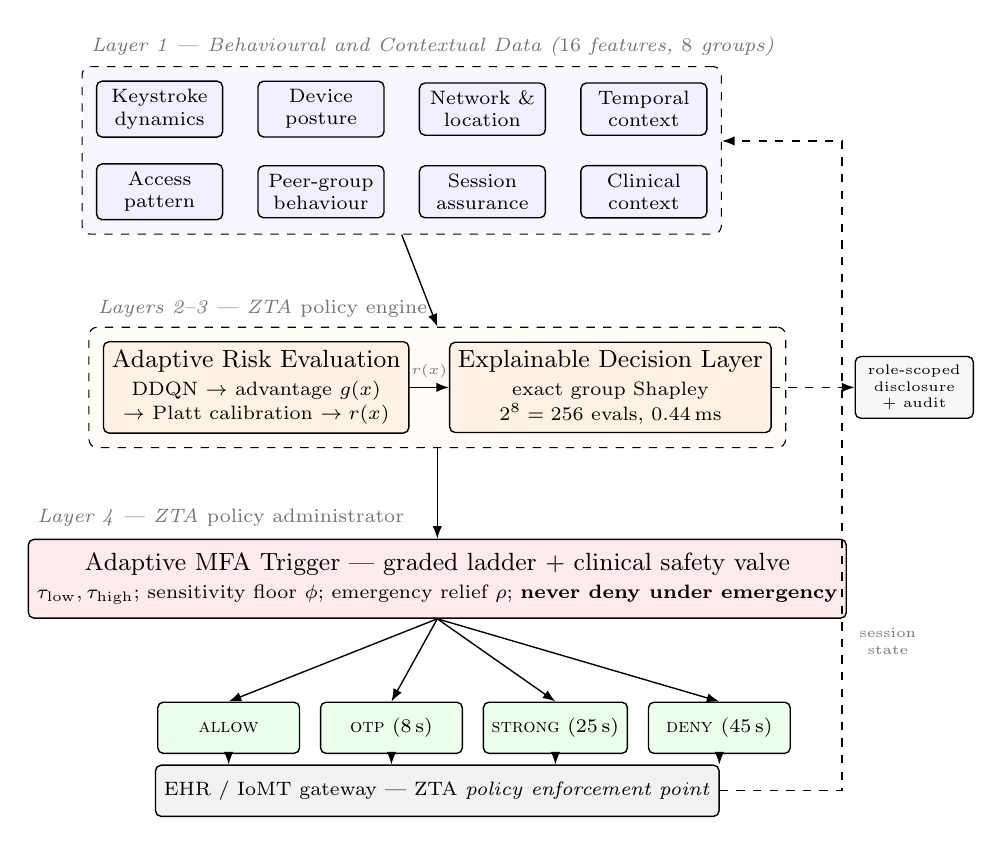
\begin{tikzpicture}[
  font=\small,
  box/.style={draw, rounded corners=2pt, align=center, minimum height=6.5mm,
              inner sep=3pt, line width=0.5pt},
  ev/.style={box, fill=blue!6, minimum width=16mm, font=\scriptsize},
  core/.style={box, fill=orange!10},
  act/.style={box, fill=green!8, minimum width=18mm, font=\scriptsize},
  lbl/.style={font=\scriptsize\itshape, text=black!55},
  ar/.style={-{Latex[length=1.6mm]}, line width=0.5pt}
]
% ---- Layer 1: evidence -------------------------------------------------
\node[ev] (g1) at (0,0)       {Keystroke\\dynamics};
\node[ev] (g2) at (2.05,0)    {Device\\posture};
\node[ev] (g3) at (4.10,0)    {Network \&\\location};
\node[ev] (g4) at (6.15,0)    {Temporal\\context};
\node[ev] (g5) at (0,-1.05)   {Access\\pattern};
\node[ev] (g6) at (2.05,-1.05){Peer-group\\behaviour};
\node[ev] (g7) at (4.10,-1.05){Session\\assurance};
\node[ev] (g8) at (6.15,-1.05){Clinical\\context};
\begin{scope}[on background layer]
\node[draw, dashed, rounded corners=3pt, fit=(g1)(g4)(g5)(g8),
      inner sep=5pt, fill=blue!3] (data) {};
\end{scope}
\node[lbl, anchor=south west] at (data.north west)
  {Layer 1 --- Behavioural and Contextual Data ($16$ features, $8$ groups)};

% ---- Layers 2-3: policy engine ----------------------------------------
\node[core, minimum width=33mm, below left=1.35cm and -0.1cm of data.south]
  (risk) {Adaptive Risk Evaluation\\[-1pt]
  {\scriptsize DDQN $\rightarrow$ advantage $g(x)$}\\[-2pt]
  {\scriptsize $\rightarrow$ Platt calibration $\rightarrow r(x)$}};
\node[core, minimum width=33mm, right=5mm of risk]
  (edl) {Explainable Decision Layer\\[-1pt]
  {\scriptsize exact group Shapley}\\[-2pt]
  {\scriptsize $2^{8}=256$ evals, $0.44$\,ms}};
\begin{scope}[on background layer]
\node[draw, dashed, rounded corners=3pt, fit=(risk)(edl), inner sep=5pt,
      fill=orange!3] (pe) {};
\end{scope}
\node[lbl, anchor=south west] at (pe.north west)
  {Layers 2--3 --- ZTA \emph{policy engine}};

% ---- Layer 4: policy administrator ------------------------------------
\node[core, fill=red!8, minimum width=71mm, minimum height=10mm,
      below=1.15cm of pe.south, anchor=north] (pa)
  {Adaptive MFA Trigger --- graded ladder $+$ clinical safety valve\\[-1pt]
   {\scriptsize $\tau_{\text{low}},\tau_{\text{high}}$; sensitivity floor
    $\phi$; emergency relief $\rho$;
    \textbf{never \deny\ under emergency}}};
\node[lbl, anchor=south west] at ([yshift=1pt]pa.north west)
  {Layer 4 --- ZTA \emph{policy administrator}};

% ---- Actions and enforcement ------------------------------------------
\node[act, below=1.05cm of pa.south, anchor=north, xshift=-26.5mm] (a1) {\allow};
\node[act, right=2.5mm of a1] (a2) {\otp\ ($8$\,s)};
\node[act, right=2.5mm of a2] (a3) {\strongauth\ ($25$\,s)};
\node[act, right=2.5mm of a3] (a4) {\deny\ ($45$\,s)};
\node[box, fill=black!5, minimum width=71mm, font=\scriptsize,
      below=0.8cm of pa.south, anchor=north, yshift=-1.05cm] (pep)
  {EHR / IoMT gateway --- ZTA \emph{policy enforcement point}};

% ---- Flow --------------------------------------------------------------
\draw[ar] (data.south) -- (pe.north);
\draw[ar] (risk) -- node[lbl, above, font=\tiny] {$r(x)$} (edl);
\draw[ar] (pe.south) -- (pa.north);
\foreach \a in {a1,a2,a3,a4} \draw[ar] (pa.south) -- (\a.north);
\foreach \a in {a1,a2,a3,a4} \draw[ar] (\a.south) -- ($(pep.north)!(\a)!($(pep.north)+(1,0)$)$);

% ---- Feedback loop (right) and disclosure (left) ----------------------
\coordinate (rt) at ($(pep.east)+(1.55,0)$);
\draw[ar, dashed] (pep.east) -- (rt) |- ($(data.east)+(0,0.12)$);
\node[lbl, font=\tiny, align=center, anchor=west, xshift=1mm]
  at ($(rt)+(0,1.9)$) {session\\state};
\node[box, fill=black!3, font=\tiny, align=center, minimum width=15mm,
      right=1.05cm of edl.east, anchor=west] (disc)
  {role-scoped\\disclosure\\$+$ audit};
\draw[ar, dashed] (edl.east) -- (disc.west);
\end{tikzpicture}}
\caption{HEAAF mapped onto the NIST zero-trust decomposition. The explanation
layer sits \emph{inside} the policy engine, so the justification exists at the
moment of the decision and is logged with it.}
\label{fig:arch}
\end{figure}

\subsection{Decision problem}

A session is a sequence of decision epochs. At epoch $t$ the engine observes
$x_t \in \mathbb{R}^{d}$, $d=16$, and selects
$a_t \in \{\allow, \otp, \strongauth, \deny\}$. The episode terminates when the
session ends, when a challenge contains an adversary, or on denial. Actions
change the state the next request is judged in --- a step-up resets the
strong-authentication clock --- so the problem is sequential rather than a
sequence of independent classifications.

Writing $Q(x,a)$ for the action-value function learned by a Double
DQN~\cite{vanhasselt2016,mnih2015}, the risk score is the calibrated advantage
of challenging over allowing,
\begin{equation}
g(x) = \max_{a \neq \allow} Q(x,a) - Q(x,\allow),
\label{eq:adv}
\end{equation}
\begin{equation}
r(x) = \sigma\!\left(w \cdot \frac{g(x)-\mu}{s} + b\right),
\label{eq:platt}
\end{equation}
where $\sigma$ is the logistic function and $(w,b)$ are fitted by Platt
scaling~\cite{platt1999} on the validation split so that the number the policy
thresholds --- and the EDL attributes --- is calibrated rather than an
arbitrary margin~\cite{guo2017}. Full reward and hyperparameter settings are in
Appendix~\ref{app:hyper}.

\subsection{Policy engine and clinical safety valve}

Let $s(x)$ denote data sensitivity and $E(x)$ flag a declared emergency
context. With $\tau_{\text{low}} < \tau_{\text{high}}$, a sensitivity floor
$\phi$ and an emergency relief term $\rho$, and writing
$\tilde r(x)= r(x) - \rho\,\mathbb{1}[E(x)]$:
\begin{equation}
a(x) =
\begin{cases}
\strongauth & \tilde r \geq \tau_{\text{high}} \wedge E(x)\\[2pt]
\deny & \tilde r \geq \tau_{\text{high}} \wedge \neg E(x)\\[2pt]
\strongauth & \tfrac{1}{2}(\tau_{\text{low}}{+}\tau_{\text{high}}) \le \tilde r < \tau_{\text{high}}\\[2pt]
\otp & \tau_{\text{low}} \leq \tilde r < \tfrac{1}{2}(\tau_{\text{low}}{+}\tau_{\text{high}})\\[2pt]
\otp & \tilde r < \tau_{\text{low}} \wedge s(x) \geq \phi\\[2pt]
\allow & \text{otherwise.}
\end{cases}
\label{eq:policy}
\end{equation}

The valve has a specific semantics: under emergency context the system may
\emph{escalate} but may never \emph{deny}. A clinician is never locked out of a
resuscitation by an automated risk score; the worst case is a second factor.
This is a structural guarantee, not an empirical tendency, and our test suite
verifies it exhaustively over the whole risk range
(Section~\ref{sec:repro}). It implements R6 directly, and
Section~\ref{sec:results-policy} isolates its effect.

\begin{algorithm}[t]
\caption{HEAAF decision cycle at one epoch}
\label{alg:cycle}
\begin{algorithmic}[1]
\Require request $x\in\mathbb{R}^{16}$; agent $Q$; head $(w,b,\mu,s)$;
         reference $\bar{x}$; thresholds $\tau_{\text{low}},\tau_{\text{high}},\phi,\rho$
\State $Q_{\text{vec}} \gets Q(x)$ \Comment{one forward pass}
\State $r \gets \sigma\!\big(w(\max_{a\neq \allow}Q_{\text{vec}}[a]-Q_{\text{vec}}[\allow]-\mu)/s + b\big)$
\State $\Phi \gets \textsc{ExactGroupShapley}(x,\bar{x})$
       \Comment{$2^{8}$ states, one batched pass}
\State $a \gets \textsc{PolicyEngine}(r, x)$ \Comment{Eq.~\eqref{eq:policy}}
\If{$E(x)$ \textbf{and} $a = \deny$} $a \gets \strongauth$
       \Comment{safety valve} \EndIf
\State $u \gets \textsc{SubjectView}(\Phi, a)$
       \Comment{one group, 3 bands, no score}
\State $v \gets \textsc{AnalystView}(\Phi, r, a)$ \Comment{full signed vector}
\State \textbf{log} $\langle x_{\text{id}}, a, r, \Phi, u\rangle$ \Comment{audit record}
\State \Return $a$, $u$
\end{algorithmic}
\end{algorithm}

\subsection{Explainable Decision Layer}
\label{sec:edl}

The EDL attributes the risk \emph{logit} rather than the probability, so
contributions combine on an additive scale, and uses a fixed clinical reference
$\bar{x}$ --- the median benign ward access --- so every explanation is
contrastive against stated routine activity rather than an uninterpretable zero
vector~\cite{aas2021}.

\paragraph{Two games, not one}
Let $N$ be the sixteen features and $v(S)=f(x_S;\bar{x}_{-S})$ the
characteristic function that switches a subset on against the reference. Exact
Shapley values over $N$ require $2^{16}=65{,}536$ evaluations. Let
$\mathcal{B}=\{B_1,\dots,B_8\}$ be the semantic partition
(Appendix~\ref{app:features}) and define the \emph{quotient game}
$\bar v(T) = v\!\left(\bigcup_{k\in T} B_k\right)$ on eight players. Exact
Shapley values of $\bar v$ require $2^{8}=256$ evaluations.

It is tempting --- and common --- to compute feature attributions and sum them
within blocks. That is not the same object. Writing $v$ in the unanimity basis
$v=\sum_T c_T u_T$, block $B$ receives $\sum_T c_T |T\cap B|/|T|$ by summation
but $\sum_{T:\,T\cap B\neq\emptyset} c_T / |\bar T|$ in the quotient game, where
$\bar T$ is the set of blocks $T$ touches. For $|T|\le 2$ these coincide for
every partition; they first diverge at $|T|=3$ when a term splits unevenly, for
instance $2c/3$ against $c/2$ for a two-one split. Both remain complete, so the
disagreement is purely in how credit is apportioned. Since a ReLU $Q$-network
carries interactions of order above two, the divergence is real here, and
Section~\ref{sec:results-edl} measures it rather than assuming it away. We
therefore report the exact quotient value as the disclosed quantity.

\paragraph{Cost}
The $256$ coalition states of one request form a single $256\times16$ matrix,
so the whole exact group attribution is one batched forward pass. This is why
exactness is affordable inline, and why it is measured
(Section~\ref{sec:results-latency}) to be cheaper than a sixteen-step
integrated-gradients approximation, which needs sixteen \emph{sequential}
backward passes.

\paragraph{Rendering}
Attributions are rendered through templates into one line of clinical English,
for example: \emph{``A one-time code was requested: the connection is coming
from an unusual place. This was the main factor in the decision.''}
Section~\ref{sec:security} explains why the subject sees one group and a band
rather than a vector and a score.

\section{Experimental Methodology}
\label{sec:method}

\subsection{Behavioural data}

The behavioural channel is real. We use the CMU keystroke-dynamics
benchmark~\cite{killourhy2009}: 51 subjects typing the password
\texttt{.tie5Roanl} 400 times across 8 sessions separated by at least 24 hours.
Sessions 1--4 enrol the per-subject template, sessions 5--6 supply training and
validation behaviour, and sessions 7--8 --- the most template-aged --- supply
test behaviour. The split therefore contains genuine template ageing rather
than a random shuffle, which is a stricter test than the shuffled evaluations
common in the keystroke literature. The verifier is the scaled-Manhattan
detector, the strongest of the fourteen algorithms in the original study; we
reproduce its error rate as a sanity check
(Section~\ref{sec:results-drift}).

\subsection{Clinical context generation}

No public corpus couples keystroke biometrics to clinical role, shift pattern,
resource sensitivity and labelled insider compromise. Contextual,
access-pattern and clinical channels are therefore generated around each real
keystroke sample by a documented generator with an explicit parameter table
(Appendix~\ref{app:hyper}), covering roles, three-shift rotas, device estates,
ward geography and resource sensitivity. Six attack scenarios are labelled and
anchored to documented incident classes (Appendix~\ref{app:attacks}).

Three properties make the testbed useful and are not obtainable from a
production access log. First, every malicious event carries a
\textbf{ground-truth driver set} --- the features the generator actually
perturbed --- so an explanation can be scored against the causal mechanism
rather than against another explainer. Second, adversaries carry a per-session
\textbf{stealth} parameter and trip only a random subset of their scenario's
drivers, so the corpus contains both loud and quiet intrusions. Third, the
benign class contains \textbf{hard negatives} --- unrostered night cover,
replacement workstations, locum first shifts, code-blue access, cross-ward
cover, remote on-call --- which are unusual \emph{and} legitimate, so a
false-positive rate measured here reflects clinical friction rather than an
easy benign baseline.

Table~\ref{tab:corpus} summarises the corpus. The malicious rate is
deliberately near $1\%$ to reflect operational base rates; accuracy is
therefore uninformative and we report G-mean, AUROC and operational friction
instead.

\begin{table}[t]
\caption{Evaluation corpus. Rates are per access event.}
\label{tab:corpus}
\centering
\small
\resizebox{\columnwidth}{!}{\input{\tablepath{tab_corpus}}}
\end{table}

\subsection{Baselines}

\begin{itemize}
\item \textbf{B1-AlwaysMFA} --- challenge every access; the maximal reading of
a mandatory-MFA rule.
\item \textbf{B2-StaticLogin} --- authenticate at the gate only; the Change
Healthcare configuration.
\item \textbf{B3-RBA} --- a Freeman-style multiplicative risk-based engine
\cite{freeman2016}, the design measured at scale by
Wiefling et al.~\cite{wiefling2022}.
\item \textbf{B4-XAI-Static} --- a supervised random forest with post-hoc
explanations, standing for the XAI-authentication
literature~\cite{raouf2024,nizam2026}.
\item \textbf{B5-RLAuth-style} --- a binary, bandit-formulated deep RL detector
without a graded policy engine and without clinical cost
terms~\cite{rlauth}.
\end{itemize}

Each baseline is evaluated with its \emph{own} native decision rule. Running a
baseline through HEAAF's policy engine would transplant the contribution under
test into the baseline and make the comparison vacuous --- indeed it makes the
baseline row numerically identical to our own detector-agnostic variant. We
additionally report budget-matched variants (suffix \texttt{@budget}) in which
the threshold is moved so the baseline spends the same clinical friction
budget, but the baseline keeps its own action mapping.

\subsection{Operating point and metrics}

Policies produce scores on incomparable scales, so comparing them at a shared
numeric threshold is meaningless. A hospital does not buy a threshold; it buys
an interruption rate. We therefore fix a \textbf{clinical friction budget} ---
the fraction of benign accesses that may be interrupted, set to $1\%$ --- read
each policy's threshold off the validation split at that budget, and report
detection at matched cost.

Beyond AUROC and G-mean we report: interrupt rate on benign traffic, interrupt
rate on hard negatives, \emph{denial rate under emergency context} (the
patient-safety failure mode), session containment rate, median epochs to
containment, expected calibration error, and an operational translation ---
department clinician-hours lost per year to authentication friction, obtained
by weighting each action by its measured clinician-facing latency
(Appendix~\ref{app:hyper}).

\subsection{Statistical protocol}
\label{sec:stats}

Two distinct sources of variability matter and are reported separately.

\emph{Training variability} is handled by repeating the entire pipeline over
$8$ independent seeds and reporting mean $\pm$ standard deviation; ablations
use $5$ seeds and the drift study $3$, for compute reasons stated in each
caption. Paired Wilcoxon signed-rank tests across seeds are reported in
Appendix~\ref{app:extra}; we note candidly that with $8$ seeds the smallest
attainable two-sided $p$ is $0.0078$, so after Holm correction over twelve
policies this test cannot reach significance for any effect, however large.
It is reported for completeness, not as the basis of any claim.

\emph{Test-sampling variability} is the binding constraint: at a $1.07\%$ base
rate a $70{,}000$-event split contains $749$ malicious events. We therefore use
a stratified paired bootstrap~\cite{efron1994} over test events, resampling
positives and negatives separately so every replicate preserves the base rate,
and pooling replicates across seeds so the resulting interval carries both
sources of variation. Because each metric compared is the mean of a $0/1$
indicator over a fixed stratum, and both policies are evaluated on the same
events, a resample is described completely by a multinomial draw over the four
joint outcome cells; sampling those counts is exactly equivalent to resampling
indices and reduces the cost from $O(n_{\text{boot}}n)$ to
$O(n_{\text{boot}})$. Multiplicity across the eight pre-specified contrasts is
controlled with Holm--Bonferroni~\cite{holm1979}, which is valid under
arbitrary dependence.
\section{Results}
\label{sec:results}

All numbers are produced by the released pipeline and written directly into
this manuscript by a generation script, so no value here is transcribed by
hand (Section~\ref{sec:repro}).

\subsection{Main comparison}
\label{sec:results-policy}

Table~\ref{tab:main} reports every policy at the $1\%$ clinical friction
budget over $8$ seeds. Fig.~\ref{fig:pareto} shows the full
security--friction frontier, which is the honest way to read a table of this
kind: any single row is one point on a curve.

\begin{table*}[t]
\caption{Main comparison at a $1\%$ clinical friction budget, mean $\pm$ s.d.\
over $8$ seeds. Bold marks the best value among policies that actually operate
at the matched budget. B1/B2 are degenerate references, not competitors. Note
that annual clinician-hours is \emph{not} monotone in interruption rate,
because the graded ladder substitutes short challenges for long denials.}
\label{tab:main}
\centering
\small
\resizebox{\textwidth}{!}{\input{\tablepath{tab_main}}}
\end{table*}

\begin{figure}[t]
\centering
\includegraphics[width=\columnwidth]{\figpath{fig_pareto.pdf}}
\caption{Security--friction frontier (3 seeds). The dotted line is the $1\%$
friction budget at which Table~\ref{tab:main} is read. The supervised detector
dominates over the whole operating range; the RL score does not.}
\label{fig:pareto}
\end{figure}

Four findings follow, and the first is a refutation of our own hypothesis.

\paragraph{The RL risk score is not the strongest detector}
Our starting position was that a reinforcement-learning agent trained with
clinically weighted rewards would learn a better risk ordering than a
supervised detector. It does not. HEAAF's RL score reaches AUROC $0.724 \pm
0.046$ against $0.960 \pm 0.001$ for the same architecture driven by a
supervised random forest, and the paired bootstrap over test events puts the
G-mean gap at $+0.378$ with a $95\%$ interval of $[0.283, 0.469]$ and
$p_{\text{Holm}}=0.002$; the TPR gap is $+0.493$ $[0.397, 0.582]$
(Table~\ref{tab:bootstrap}). The RL score is not even reliably better than a
Freeman-style statistical baseline at the same budget
($-0.080$, $[-0.170, 0.015]$, not significant).

The explanation is structural rather than a tuning failure. The supervised
detector receives a dense, per-event supervised signal; the agent receives a
sparse, delayed, heavily imbalanced reward at roughly a $1\%$ positive rate and
must simultaneously learn a ranking and a policy. What the agent \emph{is}
learning is visible in the last row of Table~\ref{tab:main}: acting greedily on
its own action-values, the agent attains the highest containment in the table
($0.966$) at an interruption rate of $41.05\%$. It has learned that challenging
is usually worth it, which is a statement about action value, not about
ranking. This is the same asymmetry Bansal and Ouda observe when they place a
supervised verifier in front of an RL controller~\cite{bansal2024}, and it is
consistent with RLAuth's own reported blind spot for attacks launched from
known environments~\cite{rlauth}.

We therefore relocate the contribution of RL to the action layer and report the
detector-agnostic variants as first-class results rather than as an appendix
curiosity.

\paragraph{The policy engine is where the value is}
Comparing rows \emph{RL agent, no policy engine} and \emph{HEAAF} isolates the
engine: the same action-values, routed through the calibrated risk head,
graded ladder and safety valve, move benign interruption from $41.05\%$ to
$1.34\%$ and annual friction from $191.8$ to $6.4$ clinician-hours. The engine
converts an unusable controller into a deployable one.

\paragraph{The safety valve removes emergency denials outright}
The cleanest test holds detector and budget fixed and varies only the policy
shape. HEAAF-SupervisedRisk and B4-XAI-Static@budget share the same random
forest, the same operating budget and the same AUROC of $0.960$. They differ
only in what the policy does with the score. Denial under declared emergency
falls from $1.099\%$ to $0.000\%$ --- a difference of $-0.0109$ with interval
$[-0.0149, -0.0072]$, $p_{\text{Holm}}=0.002$ --- for a G-mean cost of
$0.0050$ $[0.0017, 0.0095]$. Roughly one in a hundred emergency accesses is no
longer blocked by an automated risk score, at a security cost of half a
percentage point of G-mean.

HEAAF's own emergency denial rate is $0.000\%$ \emph{by construction}, not by
estimation: Eq.~\eqref{eq:policy} cannot emit \deny\ when $E(x)$ holds, and our
test suite verifies this exhaustively across the risk range and a randomised
feature space. The empirical comparison quantifies what the guarantee prevents,
it does not establish it.

\paragraph{The graded ladder is cheaper than it looks}
Annual clinician-hours are not monotone in interruption rate.
HEAAF-SupervisedRisk interrupts \emph{more} benign traffic than
B4-XAI-Static@budget ($1.53\%$ versus $1.32\%$) and reaches the same detection
($0.707$ versus $0.714$ TPR, same containment $0.904$), yet costs $7.6$ rather
than $26.5$ clinician-hours per year --- a $3.5\times$ reduction. The reason is
that the binary baseline can only deny, at $45$ measured seconds of clinician
time, whereas the graded ladder answers most elevated-risk events with an
eight-second one-time code. Two systems with the same ROC curve therefore
impose very different clinical burdens, which is an argument for reporting
operational cost alongside detection rather than instead of it.

\begin{table*}[t]
\caption{Pre-specified contrasts, stratified paired bootstrap over test events
with replicates pooled across seeds; Holm--Bonferroni over the eight rows.
Negative differences favour the first policy for emergency denials.}
\label{tab:bootstrap}
\centering
\small
\resizebox{\textwidth}{!}{\input{\tablepath{tab_bootstrap}}}
\end{table*}

\paragraph{Where the effect is not significant, we say so}
Contrasting HEAAF against its own no-valve ablation gives $-0.0012$ with
interval $[-0.0052, 0.0000]$ and no significance. This is not a failure of the
valve; it is a consequence of the weak RL score. A valve that forbids denial
only matters when the detector reaches the denial band, and the RL score
rarely does. The valve's value is therefore \emph{conditional on detector
strength}, which the B4 contrast above demonstrates directly. We prefer this
reading to the alternative of quoting only the comparison that flatters the
component.

\subsection{Calibration}

Fig.~\ref{fig:reliability} shows reliability curves. Platt scaling on the
validation split keeps expected calibration error at $0.0018$ for the RL score
and $0.0110$ for the supervised detector. Calibration matters operationally
because the friction budget is expressed as a threshold on the score: an
uncalibrated score makes the budget unenforceable, which is exactly what the
\emph{w/o risk calibration} ablation shows once thresholds are re-derived
(Section~\ref{sec:results-ablation}).

\begin{figure}[t]
\centering
\includegraphics[width=\columnwidth]{\figpath{fig_reliability.pdf}}
\caption{Reliability diagram on the test split (seed 0).}
\label{fig:reliability}
\end{figure}

\subsection{Per-scenario detection}

Table~\ref{tab:scenarios} and Fig.~\ref{fig:scenario} break detection down by
attack scenario. The ordering is informative and consistent across policies:
noisy remote credential theft is easiest ($0.972$ for the supervised
detector), and mid-session takeover is hardest ($0.352$). That ranking is a
property of the evidence, not of the classifier --- a token-theft adversary who
inherits an authenticated session on a known device from a known network
perturbs few contextual features, and the residual signal is behavioural. It
also matches the blind spot RLAuth reports for attacks from known
environments~\cite{rlauth}, and is the case where our behavioural channel
matters most.

Insider misuse ($0.558$) and IoMT gateway impersonation ($0.702$) sit between
these extremes. All three of the RL-driven policies degrade sharply on the
quieter scenarios; the RL score detects $0.441$ of credential theft but only
$0.031$ of IoMT spoofing.

\begin{table}[t]
\caption{Per-scenario detection rate at the $1\%$ budget, mean over $8$ seeds.
The last column is the rate at which the top-3 feature attribution recovers at
least one ground-truth driver of that scenario (IG-16).}
\label{tab:scenarios}
\centering
\scriptsize
\resizebox{\columnwidth}{!}{\input{\tablepath{tab_scenarios}}}
\end{table}

\begin{figure*}[t]
\centering
\includegraphics[width=\textwidth]{\figpath{fig_per_scenario.pdf}}
\caption{Detection rate by attack scenario at a matched friction budget; error
bars are standard deviation over $8$ seeds.}
\label{fig:scenario}
\end{figure*}

\subsection{The explanation need not be approximate}
\label{sec:results-edl}

This is the result we consider most transferable beyond authentication.

Table~\ref{tab:explanations} is the conventional picture at the level of
sixteen features: exact Shapley costs $57.2$\,ms, and every practical method is
an approximation on a cost--fidelity frontier. KernelSHAP-512 reaches
$\rho=0.820$ at $4.86$\,ms; integrated gradients reach $\rho \approx 0.62$ at
$0.016$--$0.058$\,ms. Grad$\times$Input is fastest, least faithful
($\rho=0.544$), and has a completeness gap of $4.75$ --- it does not decompose
the score it claims to explain.

Table~\ref{tab:group} is the picture at the level a clinician actually reads,
and it is qualitatively different. Exact Shapley over the eight semantic groups
costs $1.87$\,ms measured per explanation in this benchmark, and $0.44$\,ms at
the median when batched on the decision path
(Table~\ref{tab:latency}). Exactness is not a reference point here; it is the
cheapest faithful option, and it is what HEAAF discloses.

\begin{table}[t]
\caption{Feature-level attribution fidelity against exact Shapley over
$2^{16}$ coalitions ($300$ instances, seed 0). Stability is the mean $L_2$
change under $\sigma{=}0.01$ input noise (lower is better) and is reported in
Appendix~\ref{app:extra}.}
\label{tab:explanations}
\centering
\scriptsize
\resizebox{\columnwidth}{!}{\input{\tablepath{tab_explanations}}}
\end{table}

\begin{table}[t]
\caption{Group-level attribution: the quantity actually disclosed. Fidelity is
measured against \emph{exact group Shapley} over $2^{8}$ coalitions
($500$ instances, seed 0).}
\label{tab:group}
\centering
\scriptsize
\resizebox{\columnwidth}{!}{\input{\tablepath{tab_group}}}
\end{table}

\begin{figure*}[t]
\centering
\includegraphics[width=\textwidth]{\figpath{fig_explanation_frontier.pdf}}
\caption{Cost against fidelity. (a) At the feature level exactness is a
$57$\,ms reference point and every method is an approximation. (b) At the group
level --- the disclosed quantity --- exactness costs $1.9$\,ms in this
benchmark and dominates every approximation. Block-summed exact feature
Shapley is $28\times$ more expensive \emph{and} disagrees with the group value
it is meant to stand in for.}
\label{fig:frontier}
\end{figure*}

\paragraph{Block sums are not group Shapley values}
Summing exact feature-level Shapley values into blocks --- the standard
shortcut --- attains Spearman $\rho = 0.928$ against the exact group value,
recovers the dominant group in only $87.0\%$ of cases, and carries relative
$L_1$ error $0.203$, while costing $53.3$\,ms against $1.87$\,ms. Both
quantities are complete, so this is not an approximation error in the usual
sense: it is a genuine disagreement about how credit is apportioned, exactly as
Section~\ref{sec:edl} predicts once interactions of order three or above
straddle groups unevenly. Practitioners who aggregate SHAP values into
feature groups for readability should be aware that they are reporting a
different quantity from the group Shapley value, and that in this system the
two disagree on the headline factor roughly one time in eight.

\paragraph{Approximation degrades faster at the group level}
Integrated gradients transfer poorly under aggregation: IG-32 falls from
$\rho=0.620$ at the feature level to $\rho=0.629$ against the group ground
truth with top-1 agreement of only $0.604$, and its completeness gap
($0.252$) is now visible against a target that has none. Since the disclosed
statement names \emph{one} group, top-1 agreement is the operationally relevant
figure, and $0.604$ means a cheap explainer would name the wrong dominant
factor in two cases out of five.

\paragraph{Do the explanations point at the true cause?}
Because the generator records which features each attack perturbs, attribution
can be scored against the causal mechanism rather than against another
explainer. The exact group attribution names a true driver group as the single
dominant factor in $69.7\%$ of malicious events and places one in its top two
in $84.7\%$. At the feature level, the top-3 attribution recovers at least one
declared driver for $91.1\%$ of malicious events overall, ranging from
$85.7\%$ (insider misuse) to $100\%$ (mid-session takeover)
(Table~\ref{tab:scenarios}). Fig.~\ref{fig:signature} shows that the mean
attribution signature differs per scenario in the direction the generator
intends --- session assurance dominates IoMT spoofing, peer-group deviation
dominates mid-session takeover, access pattern dominates insider misuse ---
which is the property an investigator needs when triaging an alert.

\begin{figure*}[t]
\centering
\includegraphics[width=\textwidth]{\figpath{fig_group_signature.pdf}}
\caption{Mean exact group attribution per attack scenario, normalised per row.
Red is evidence for challenge. Signatures separate in the direction the
generator's driver sets specify.}
\label{fig:signature}
\end{figure*}

\subsection{Decision-path latency}
\label{sec:results-latency}

Table~\ref{tab:latency} reports the measured cost of each stage on a single
CPU core.

\begin{table}[t]
\caption{Decision-path latency over $200$ repetitions, single CPU core, no
GPU. The exact group attribution is a single batched forward pass over $256$
coalition states.}
\label{tab:latency}
\centering
\small
\resizebox{\columnwidth}{!}{\input{\tablepath{tab_latency}}}
\end{table}

The headline is that \textbf{the exact explanation is cheaper than the
approximate one}. A complete end-to-end decision --- score, explain, apply
policy --- costs $0.611$\,ms at the median with exact group Shapley and
$1.214$\,ms with sixteen-step integrated gradients. The reason is
architectural rather than algorithmic: the $256$ coalition states of a group
attribution form one $256\times16$ matrix and are scored in a single batched
forward pass, whereas integrated gradients require sixteen \emph{sequential}
gradient evaluations whose per-call overhead dominates at batch size one. At
p99 the exact path costs $0.748$\,ms, leaving three orders of magnitude of
headroom against the $\sim$$500$\,ms threshold at which interface latency
becomes perceptible. Explanation is therefore not the bottleneck in this
design, and there is no efficiency argument for disclosing an approximation.

\subsection{Ablations}
\label{sec:results-ablation}

Table~\ref{tab:ablation} and Fig.~\ref{fig:ablation} remove one component at a
time. Every arm is given the threshold that spends the same $1\%$ friction
budget on validation, so the comparison is ``same cost to clinicians, how much
security do you get''. This matters: an earlier version of this experiment
compared arms at a \emph{fixed} threshold, which conflated components that
improve ranking with components that merely shift the score distribution, and
made the no-calibration arm appear to interrupt $98\%$ of benign traffic when
it was in fact measuring the threshold rather than the ablation.

\begin{table}[t]
\caption{Component ablations at a matched $1\%$ friction budget, mean $\pm$
s.d.\ over $5$ seeds.}
\label{tab:ablation}
\centering
\small
\resizebox{\columnwidth}{!}{\input{\tablepath{tab_ablation}}}
\end{table}

\begin{figure}[t]
\centering
\includegraphics[width=\columnwidth]{\figpath{fig_ablation.pdf}}
\caption{Change in G-mean when each component is removed, at a matched
friction budget. Error bars are standard deviation over $5$ seeds.}
\label{fig:ablation}
\end{figure}

Both evidence channels contribute, and the contextual channel contributes more
($\Delta = -0.221$) than the behavioural channel ($\Delta = -0.113$). This is
consistent with the per-scenario results: four of six scenarios are primarily
contextual. It also supports R5 --- neither channel alone is sufficient.
Sequential credit assignment contributes modestly ($\Delta=-0.015$), which is
weaker evidence for the sequential formulation than we expected and is
consistent with the finding that the RL layer is not where detection comes
from.

Three arms deserve honest comment because they do \emph{not} support the
design.

\emph{Removing the graded ladder improves G-mean} ($\Delta=+0.034$). Collapsing
four actions to allow/deny concentrates the same friction budget into denials,
which contain more sessions. G-mean does not see the cost of doing so; the
clinician-hours column and the emergency-denial column do. This is precisely
why we report operational cost separately, and it is a caution against
optimising a single scalar.

\emph{Removing clinical cost terms} also nudges G-mean up ($+0.010$, well
inside one standard deviation). The reward's clinical weighting buys
patient-safety behaviour, not raw separability, and G-mean is the wrong
instrument for detecting it.

\emph{Removing risk calibration} changes G-mean by $-0.000$. Once thresholds
are budget-matched, calibration is a monotone reparameterisation and cannot
change the ranking. Its value is that the budget becomes \emph{expressible} at
all, and that the number the EDL attributes is a probability rather than an
arbitrary margin --- neither of which G-mean measures. We report the null
result rather than dropping the arm.

The safety-valve arm is the only one that moves the patient-safety metric:
emergency denials rise from $0.000\%$ to $0.080\%$ when it is removed, at
essentially unchanged G-mean.

\subsection{Template ageing}
\label{sec:results-drift}

Behavioural templates decay. Table~\ref{tab:drift} and Fig.~\ref{fig:drift}
quantify it by enrolling on sessions 1--4 and testing on progressively later
sessions.

\begin{table}[t]
\caption{Template ageing. Keystroke EER is the scaled-Manhattan verifier
enrolled on sessions 1--4; G-mean columns are end-to-end at a $1\%$ budget,
mean $\pm$ s.d.\ over $3$ seeds.}
\label{tab:drift}
\centering
\small
\resizebox{\columnwidth}{!}{\input{\tablepath{tab_drift}}}
\end{table}

\begin{figure*}[t]
\centering
\includegraphics[width=\textwidth]{\figpath{fig_drift.pdf}}
\caption{(a) Keystroke EER rises monotonically as the gap between enrolment
and test widens. (b) The end-to-end effect is muted because contextual
evidence does not age on the same clock.}
\label{fig:drift}
\end{figure*}

Two observations. First, the behavioural channel degrades monotonically, from
EER $0.0825$ at session~5 to $0.1028$ at session~8 --- a relative increase of
$24.6\%$ across four sessions. Our session-7--8 figure of $\approx 0.10$ is
consistent with the $\approx 0.096$ that Killourhy and Maxion report for
scaled Manhattan~\cite{killourhy2009}, which is the sanity check that our
behavioural channel is wired up correctly; we make this a unit test rather than
a claim (Section~\ref{sec:repro}).

Second, the end-to-end effect is far smaller than the channel-level effect:
HEAAF's G-mean moves within its seed noise across session blocks. Multi-channel
fusion absorbs behavioural decay because contextual, temporal and
access-pattern evidence do not age on the same clock. This is an argument for
fusion, and simultaneously a caution: a system that relied on keystroke
evidence alone would require re-enrolment on a schedule this experiment
suggests is measured in weeks.
\section{The Explanation Channel as an Attack Surface}
\label{sec:security}

Every explanation returned to a challenged user is information returned to
whoever is at the keyboard, adversary included. The XAI-authentication
literature does not treat this as a design constraint~\cite{raouf2024,nizam2026},
but the wider XAI-security literature is unambiguous that it should be:
attributions leak membership~\cite{shokri2021}, Shapley vectors permit
reconstruction of private inputs~\cite{luo2022}, post-hoc explainers can be
actively fooled~\cite{slack2020}, and the surface is now
surveyed~\cite{baniecki2024,nguyen2024,quan2022}.

Authentication is the sharper case. Unlike a loan applicant, an adversary
against a continuous-authentication system controls the very features being
attributed, can issue many probes, and receives feedback each time. A signed,
per-feature attribution vector paired with a numeric score is close to a
gradient oracle: it identifies which coordinate to change and in which
direction. Repeated probing then reduces evasion to hill-climbing --- the
threat model Agrawal et al.\ demonstrate against touch-based continuous
authentication~\cite{agrawal2021}.

HEAAF resolves the tension between the transparency duty and this leakage by
refusing to emit one explanation. The same attribution vector is projected
differently for each audience:

\begin{itemize}
\item \textbf{Subject (the clinician being challenged).} One dominant semantic
group, named in clinical English, with a three-level magnitude band and
\emph{no numeric score}. Measured over the test instances, this releases $1$
coordinate of $8$, carries at most $\log_2(8\times3)=4.58$ bits per decision,
and the named group accounts for $56.9\%$ of the positive attribution mass ---
so more than two-fifths of the evidence is not disclosed at all.
\item \textbf{Analyst (SOC / information governance).} The complete signed
eight-vector, the calibrated score and the reconciliation against the clinical
reference.
\item \textbf{Audit record.} Everything, written at decision time. Because the
justification is generated inside the decision cycle
(Fig.~\ref{fig:arch}), it cannot later be reconstructed from a retrained
model --- which is what makes it admissible as a record of why \emph{that}
decision was taken.
\end{itemize}

Three caveats. First, coarsening reduces the leak rate; it does not eliminate
it, and an adversary who can force many challenges still accumulates
information. Rate-limiting disclosure per subject per interval is a natural
companion control and is not evaluated here. Second, we quantify the channel
but do not run an adaptive adversary against it; constructing one is the most
important piece of future work this design implies. Third, coarsening trades
against the GDPR Article 22 interest in meaningful information about automated
decision-making~\cite{gdpr}: our position is that the subject receives a
meaningful reason and the regulator receives the complete record, but this is a
defensible design choice rather than a settled legal question.

\section{Governance and Regulatory Alignment}

Under the EU AI Act~\cite{euaiact}, a system of this kind used in a clinical
setting is plausibly high-risk, attracting obligations on risk management,
logging, transparency and human oversight. Three properties of the design
address these directly. Attributions are generated at decision time and stored
with the decision, satisfying record-keeping without post-hoc reconstruction.
The graded ladder and safety valve keep a human in the loop by construction:
the system's strongest action against a clinician in an emergency is to request
a second factor, never to refuse. Role-scoped disclosure separates the
transparency duty to the data subject from the completeness duty to the
regulator.

Under UK GDPR and the NHS Data Security and Protection
Toolkit~\cite{nhsdspt}, per-decision attributions provide the evidence trail
that access controls are risk-proportionate. HHS OCR's proposed removal of the
``addressable'' designation for MFA~\cite{hhsnprm} would make continuous,
context-aware authentication a compliance question and not only an engineering
one; we note it remains proposed rather than final as of this writing.

\section{Limitations and Threats to Validity}
\label{sec:limits}

We state these plainly, since several bear directly on how far the results
generalise.

\textbf{The clinical context is generated.} The behavioural channel is the real
CMU corpus with a genuine ageing split, but role, shift, device, geography,
resource sensitivity and attack labels are produced by a parameterised
generator. Absolute rates are therefore properties of the generator, not
estimates of hospital reality, and should not be quoted as such. What the
testbed supports is \emph{relative} comparison under identical conditions,
which is what every claim in Section~\ref{sec:results} is. Ground-truth driver
sets --- the basis of our attribution-grounding results --- are obtainable in no
other way we know of; a production access log does not record which features an
attacker perturbed.

\textbf{Generator--detector circularity.} Detectors are evaluated on data whose
generative process is known to us. We mitigate this with per-session stealth
parameters, partial driver activation and a hard-negative class designed to be
unusual but legitimate, but the mitigation is partial. The absolute detection
rates in Table~\ref{tab:main} would be optimistic on real traffic.

\textbf{Single behavioural modality.} The CMU corpus is fixed-text password
typing on a desktop keyboard. Clinical workflows involve tablets, shared
workstations, gloved hands and voice; free-text and touch dynamics carry
different error characteristics, and our conclusions about the behavioural
channel do not automatically transfer.

\textbf{No adaptive adversary.} Attacks are drawn from a fixed taxonomy and do
not respond to the defence. Given that we return explanations to the person
being challenged, an adaptive-adversary evaluation is the single most important
missing experiment (Section~\ref{sec:security}).

\textbf{Seed count.} Eight seeds is enough for a stable mean but is a small
sample for a rank test; as noted in Section~\ref{sec:stats}, the seed-level
Wilcoxon test cannot reach corrected significance at this sample size and no
claim rests on it. All significance claims come from the event-level bootstrap.

\textbf{Not compared to RLAuth's published number.} RLAuth reports G-mean
$92.62\%$~\cite{rlauth}; our RLAuth-style baseline reaches $0.383$ at a matched
budget. These numbers are not comparable and we do not present them as such:
different data, a different base rate, a different action space and a
different threat model. Our B5 is a faithful reimplementation of the
\emph{formulation} --- binary, bandit-style, no clinical cost terms --- evaluated
on our corpus, not a reproduction of their result.

\textbf{Cost parameters are illustrative.} Clinician-seconds per action and
breach costs are plausible published estimates, not measurements from a
partner site. The conclusion that the graded ladder reduces friction cost by
$3.5\times$ depends on the ratio between challenge and denial time, which we
report explicitly (Appendix~\ref{app:hyper}) so it can be re-derived under
different assumptions.

\section{Conclusion}

We set out to build an adaptive continuous-authentication system that could
justify itself inside the decision cycle and price patient safety explicitly,
and we tested the hypothesis that reinforcement learning would supply the
detection.

That hypothesis was wrong, and we report it as such. A supervised detector
inside the same policy engine gains $0.378$ G-mean $[0.283, 0.469]$ over the
RL-derived score. The contribution of the RL formulation lies in the action
layer: routed through the calibrated head, graded ladder and safety valve, the
same agent goes from interrupting $41.05\%$ of benign traffic to $1.34\%$.

Two positive results stand. First, the explanation disclosed to a clinician
need not be an approximation. Because sixteen evidence features partition into
eight semantic groups, exact group-level Shapley values cost $256$ coalition
evaluations, run in $0.44$\,ms, and make a complete end-to-end decision with an
exact justification \emph{cheaper} ($0.611$\,ms) than the same decision
explained approximately ($1.214$\,ms). We also show that the common practice of
summing feature attributions into groups is a different quantity from the group
Shapley value, disagreeing on the dominant factor about one time in eight ---
a caution that applies wherever attributions are aggregated for readability.
Second, an explicit clinical safety valve eliminates emergency denials: holding
detector and friction budget fixed, denial under declared emergency falls from
$1.099\%$ to $0.000\%$ for $0.005$ G-mean, and the graded ladder delivers the
same detection at $7.6$ rather than $26.5$ clinician-hours of annual friction.

The wider lesson is that in clinical security the policy layer, not the
classifier, is where safety is won or lost --- and that a system which must
explain itself to the person it is challenging should decide, in advance, how
much it is willing to say.

\section*{Reproducibility}
\label{sec:repro}

The implementation, generator, evaluation harness and figure and table scripts
are released. Three properties are worth noting for a reader wishing to check
the argument mechanically.

\emph{Numbers cannot drift.} Every table in this paper is emitted by
\texttt{scripts/make\_tables.py} directly from the persisted result files and
input as a \LaTeX{} fragment; no value is transcribed by hand. Re-running the
pipeline and the script regenerates the manuscript's numbers.

\emph{The argument's premises are unit-tested.} A suite of $35$ invariant tests
(\texttt{pytest -q}) checks the properties the paper's claims rest on rather
than merely exercising the code: that exact Shapley satisfies efficiency,
symmetry and the dummy axiom and matches the closed form on a linear model;
that group and feature games coincide under pairwise interaction and diverge
under three-way interaction, as Section~\ref{sec:edl} argues; that the safety
valve never denies a declared emergency, checked exhaustively over the risk
range; that the policy is monotone in risk; that the subject disclosure never
contains the numeric score and never names more than one group; and that the
scaled-Manhattan verifier reproduces the published EER range.

\emph{Staged and resumable.} \texttt{scripts/stage.py} runs each stage
independently against persisted artefacts, so a reviewer can re-run one
experiment without repeating the whole pipeline.

\balance
\bibliographystyle{IEEEtran}
\bibliography{refs}

\appendices

\section{Feature Space and Semantic Groups}
\label{app:features}

Table~\ref{tab:features} lists the sixteen features and the partition into
eight semantic groups used throughout. The partition is mutually exclusive and
jointly exhaustive; this is asserted at import time and unit-tested, because
the exactness and completeness guarantees of Section~\ref{sec:edl} depend on
it.

\begin{table*}[t]
\caption{The sixteen evidence features and their partition into eight semantic
groups. Group membership is the unit at which the clinician-facing disclosure
is made.}
\label{tab:features}
\centering
\small
\resizebox{\textwidth}{!}{\input{\tablepath{tab_features}}}
\end{table*}

\section{Attack Taxonomy and Hard Negatives}
\label{app:attacks}

Table~\ref{tab:attacks} lists the six attack scenarios, their mix weights,
the documented incident class each is anchored to, and the ground-truth driver
features the generator perturbs. Adversaries carry a per-session stealth
parameter and activate only a random subset of their driver set, so the corpus
contains both loud and quiet intrusions. Hard negatives are legitimate
behaviours constructed to trip similar features, and are the reason the
false-positive rates reported in Section~\ref{sec:results} correspond to
clinical friction rather than to an easy benign baseline.

\begin{table*}[t]
\caption{Attack scenarios and hard negatives. Driver features are the
ground truth against which attributions are scored in
Section~\ref{sec:results-edl}.}
\label{tab:attacks}
\centering
\small
\resizebox{\textwidth}{!}{\input{\tablepath{tab_attacks}}}
\end{table*}

\section{Reward Model and Hyperparameters}
\label{app:hyper}

The reward encodes the clinical asymmetry that motivates the whole design. A
missed compromise costs $-(\,\text{breach\_base} + \text{gain}\times s(x))$,
scaling with data sensitivity. A frictionless allow on benign traffic earns a
small positive reward, so the agent is not rewarded for blanket suspicion.
Challenges carry a friction penalty graded by clinician time, and an
\emph{additional} penalty when the context is a declared emergency, with denial
penalised far more heavily than a one-time code. Correctly challenging a
compromised session earns a positive reward graded by how much of the session
remains to be contained.

Clinician-seconds per action ($8$\,s for a one-time code, $25$\,s for strong
re-authentication, $45$\,s for a denial including the recovery path) are the
basis of the annual clinician-hour column in Table~\ref{tab:main} and are the
parameter to vary if local measurements differ.

\begin{table*}[t]
\caption{Complete hyperparameter and cost settings. All values are defaults in
the released configuration.}
\label{tab:hyper}
\centering
\small
\resizebox{\textwidth}{!}{\input{\tablepath{tab_hyper}}}
\end{table*}

\section{Supplementary Results}
\label{app:extra}

\paragraph{Attribution stability}
The stability column of Table~\ref{tab:explanations} measures the mean $L_2$
change in the attribution vector under Gaussian input perturbation with
$\sigma = 0.01$. Exact Shapley is the most stable ($2.56$), consistent with its
averaging over all coalitions. KernelSHAP-128 is the least stable ($14.63$),
because sampling noise adds to model curvature; increasing the sample budget to
$512$ roughly halves it ($7.48$). Grad$\times$Input is unstable ($9.77$) for a
different reason: it reads a single local gradient, so it inherits the
curvature of the ReLU network directly. Stability matters operationally because
an explanation that changes materially between two near-identical requests
cannot be defended in an audit.

\paragraph{Training dynamics}
Fig.~\ref{fig:training} shows episode return and temporal-difference loss
across seeds. Returns converge within roughly $40{,}000$ environment steps and
the spread across seeds is visible in the standard deviations of
Table~\ref{tab:main}; the RL-driven rows carry seed standard deviations an
order of magnitude larger than the supervised rows ($0.055$ against $0.003$ in
G-mean), which is itself part of the case that the RL layer is not where
detection should come from.

\begin{figure*}[t]
\centering
\includegraphics[width=\textwidth]{\figpath{fig_training.pdf}}
\caption{Double-DQN training dynamics across seeds.}
\label{fig:training}
\end{figure*}

\paragraph{Seed-level paired tests}
For completeness we report the paired Wilcoxon signed-rank comparison of every
policy against HEAAF across the $8$ seeds in the released
\texttt{table\_significance.csv}. As stated in Section~\ref{sec:stats}, with
$n=8$ the smallest attainable two-sided $p$ is $2/2^{8} = 0.0078$, so after
Holm correction across twelve policies no comparison can reach $\alpha=0.05$
regardless of effect size. Uncorrected, the large effects
(HEAAF-SupervisedRisk, HEAAF-Ensemble, RL-argmax, B4-XAI-Static@budget) all
attain the floor value of $0.0078$, and the direction of every one agrees with
the corresponding bootstrap interval in Table~\ref{tab:bootstrap}. We rest no
claim on this test and report it only so the reader can see that the two
instruments agree.

\paragraph{A worked disclosure}
For a mid-session takeover event with calibrated risk $0.71$, the exact group
attribution is dominated by peer-group behaviour and device posture. The
subject sees: \emph{``A one-time code was requested: the activity differs from
others in your role. This was the main factor in the decision.''} The analyst
sees the full signed vector, the score, and the reconciliation against the
clinical reference. The audit record stores both, plus the reason code, at
decision time.

\end{document}
